\documentclass[a4paper]{article}
\usepackage{amsmath,epsfig}
\usepackage{algorithmicx,algorithm}
\usepackage{algpseudocode}
\usepackage{multirow}
\usepackage{array}
\usepackage{graphicx}
\usepackage{subfigure}
\usepackage{amsmath}
\usepackage{booktabs}
\usepackage{subfigure}
\usepackage{amsmath}
\usepackage{booktabs}
\usepackage{bm}
\usepackage{caption}
\usepackage{INTERSPEECH2021}

\title{An Adaptive Few-Shot Learning  Algorithm for Rare Sound Event Detection}
\name{Leilai Li, Jianzong Wang*\thanks{* Corresponding author: Jianzong Wang, jzwang@188.com.}, Xiaoyang Qu, Chendong Zhao, Jing Xiao}
\address{Ping An Technology (Shenzhen) Co., Ltd.}
\email{\{lileilai446,wangjianzong347,quxiaoyang343,\\
	zhaochendong343,xiaojing661\}@pingan.com.cn}

\begin{document}

\maketitle 
\begin{abstract}
  Sound event detection is to infer the event by understanding the surrounding environmental sounds. 
  Few-shot learning methods promise generating a well-trained model which is easily generalized when facing a new limit-data sound detect task without many training steps. 
  Recent approaches have achieved significant results in this field. However, these approaches treat each support example independently ignoring the information of other examples (events) from the whole task. 
  Because of this, most of previous methods are constrained to generate a same feature embedding facing all test-time tasks. An ideal model would construct a feature embedding adapted to the input task. 
  In this work, we propose a novel task-adaptive module which is easily ported to any metric-based few-shot learning frameworks. The module could identify the task-relevant feature dimension. Incorporating our module improves performance considerably on two datasets over baseline methods, especially for the transductive propagation network. Such as +6.8\% for \textit{5-way 1-shot} accuracy on ESC-50, and +5.9\% on noiseESC-50. We also investigate our approach in the domain-mismatch setting and achieve better results than previous methods.
\end{abstract} 
\noindent\textbf{Index Terms}: Sound event detection, Few-shot learning, Data augmentation, Deep learning

\section{Introduction}
\label{sec:intro}

Automatic environmental sound event detection has received increasing attention in recent years~\cite{TUTDatatbase}. It deals with audios detecting and classifying, which leads to multi-form applications in industry. Environmental sound is naturally different from other audios. It doesn't exhibit any stationary temporal patterns like phoneme in speech or rhythm in music. In contrast, sound event contains very complex temporal structure~\cite{sed1,sed2,se} that may be continues (e.g. rains), abrupt (e.g. thunder storm) or periodic (e.g. clock tick). Moreover, speech and music usually distribute on a relatively fixed frequency bandwidth, but sound event spans a wide frequency range where different sound’s frequency may distribute in various patterns~\cite{su2017weakly,pert}. The information contained in temporal patterns and frequency bins of the sound event could be massive~\cite{tf}.

To date, many deep-learning (DL) methods greatly improved detection performance~\cite{autoTagging,audiofew,song,park,few-shot-sound-detection}. However, they typically require large amounts of labeled data, which limits the generalization ability to limited-data tasks due to the annotation cost. These motivate the study of \textbf{Few-shot learning}. Meantime, this method has also been introduced in ~\cite{attentionSimilarity,rare,few-att-gnn,fewShotGNN,TPN} which concerning rare sound event detection and achieved promising results. Few-shot model promises alleviating the problem of data deficit and cold start. It usually follows the episodic training strategy~\cite{attentionSimilarity,MatchNet}, which considers an N-way K-shot (e.g 5 way, 1 shot means there’re 5 classes, each contains 1 support example) classification task in each episode.
\begin{figure}[t]
	\centering
	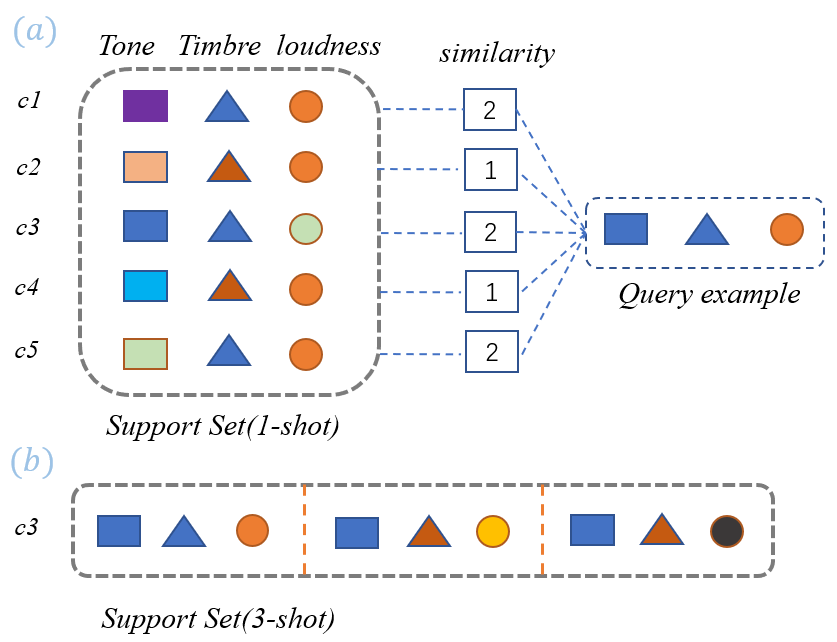
\includegraphics[width=0.95\linewidth]{./pic/idea-3.png}
	\caption{An example illustrates the motivation. (a) defines a 5-way 1-shot task. There’re three feature dimensions: \textit{Tone}, \textit{Timbre} and \textit{loudness}. Different color means different value of the feature, same color adds the similarity score by 1; (b) In the k-shot (k=3) setting, all examples of class c3 share the same value of \textit{Tone} even though their \textit{Timbre} and \textit{loudness} are different. }
	\label{fig:idea}
	\vspace{-4mm}
\end{figure}


All metric-based few-shot learning frameworks~\cite{fewShotGNN, TPN, protoNet, relationNet, CloserLook} compute similarity between each support (training) example and the query example independently, resulting in the correlation among support examples being missed. Figure~\ref{fig:idea} illustrates our motivation of the task-adaptive module. Each support example has different \textit{Tone}, but may have same \textit{Timbre} and \textit{loudness} with others. During the similarity computation, the score between support example (c1, c3, c5) and the query example are all 2, making it hard to classify the query example. Moreover, in multi-shot setting like Figure~\ref{fig:idea} (b) shows, most of class c3 have the same \textit{Tone} but various \textit{Timbre} and \textit{loudness}. Above all, the critical feature in this task should be \textit{Tone}. Our task-adaptive module aims to integrate all support examples' information to value the commonality within per class and the uniqueness among all classes, thus to find the critical features. 

Our contributions are as follows: 
(1) We introduce a feature encoder integrating attention mechanism to capture the temporal\&channel context. In addition, a sound event-oriented data augmentaion strategy is introduced to alleviate the data-shortage problem. 
(2) We extend metric-based few-shot learning frameworks with a task-adaptive module to identify the uniqueness among classes and the commonality within per class of the whole support set. The task-adaptive module makes the feature-embedding process more effective. (3) We evaluated our model on two benchmarks. Results verify the superiority of our model over previous methods. Besides, our model also achieves better performance in the setting of domain mismatch.

\begin{figure*}[t]
	\centering
    \vspace*{-12mm}
	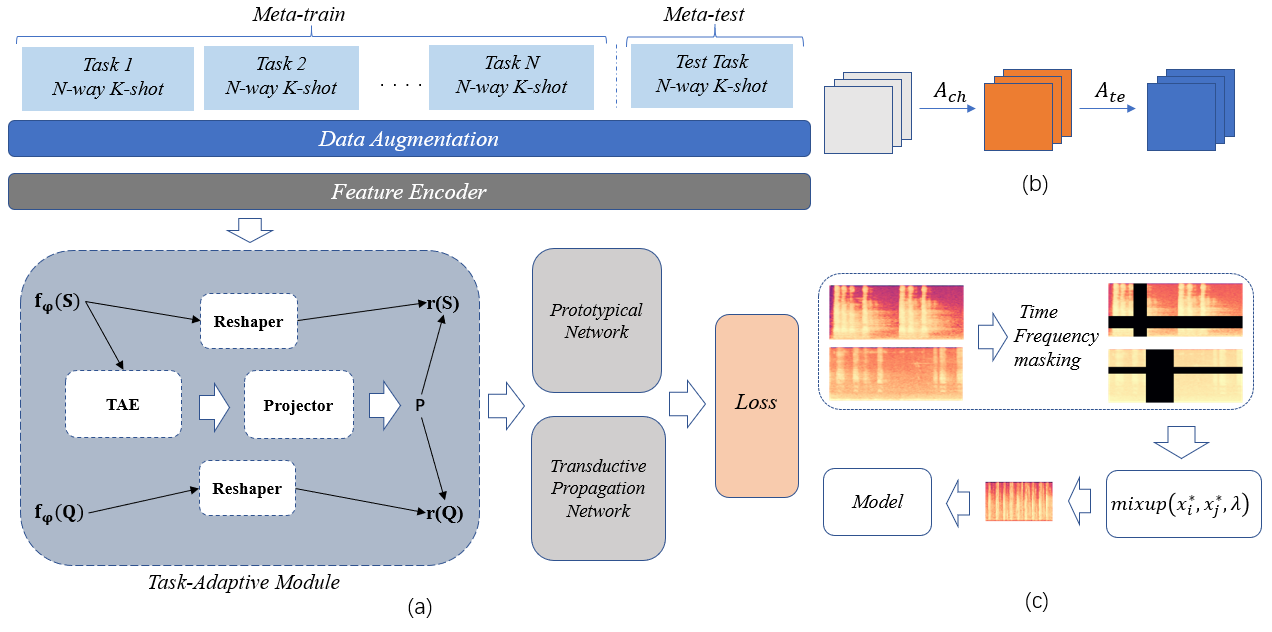
\includegraphics[width=\linewidth]{./pic/model.png}
	\vspace*{-6mm}
	\caption{(a). The overall framework of our model, it is composed of three parts: feature encoder, task-adaptive module and metric-based few-shot learning network. (b). The temporal\&channel attention mechanism. $A_{ch}$ is the channel attention, $A_{te}$ is the temporal attention. (c). Data augmentation pipeline for the input log mel-spectrogram.}
	\label{fig:model}
	\vspace*{-3mm}
\end{figure*}


\section{Preliminary}

\subsection{Few-shot sound event detection}
\vspace{-1.5mm}
Recent approaches~\cite{audiofew,attentionSimilarity,few-att-gnn} adopt the prototypical networks~\cite{protoNet} and graph neural networks~\cite{fewgnn} for few-shot sound event detection. Few-shot sound event detection aims to correctly classify unlabeled sounds with a few labeled examples.

Few-shot learning follows the episodic training paradigm that used in previous literature \cite{protoNet,maml}. Supposing there're two non-overlapping
datasets of classes (events) $\bm{C}_{train}$ and $\bm{C}_{test}$, where $\bm{C}_{train} \cap \bm{C}_{test} = \emptyset$. There are also two procedures: meta-training and meta-testing. In one episode of training, we randomly sample $N$ classes (a small subset) from $\bm{C}_{train}$ to construct support set $\mathcal{S}$ and query set $\mathcal{Q}$. A simple $N$-way $K$-shot task denotes as follow: $\mathcal{S}$ is denoted as $\mathcal{S} = \{x_1^1,...,x_K^1,..,x^N_1,..,x^N_K\}$, where $K$ is the number of samples in per class. The query set $\mathcal{Q} = \{ x_1^*,...,x_T^*\}$ contains various examples from the same $N$ classes. Thus, there are $NK$ samples in $\mathcal{S}$ and $T$ samples in $\mathcal{Q}$.  The support set and query set composed a multi-label classification task here. During the procedure of meta-testing, $\mathcal{S}$ and $\mathcal{Q}$ sampled from $\bm{C}_{test}$ , and few-shot method is required to predict on query set (no label) given the support set (with label).

\vspace{-2mm}
\subsection{Metric-based learning methods}
\label{methods}
\vspace{-1.5mm}
Few-shot learning methods can be divided into three branches: metric-based, optimization-based and data augmentation-based~\cite{opt1,opt2,koch2015siamese}. In this paper, we mainly focus on metric-based learning. The metric-based methods could be categorized into inductive and transductive, and two representative methods are prototypical network~\cite{protoNet} and transductive propagation network (\textit{TPN})~\cite{TPN}.
Given a $N$-way $K$-shot task $\mathcal{T} = (\mathcal{S}, \mathcal{Q})$, and the feature encoder $f_\varphi$ decided by its internal parameter $\varphi$.

\textbf{Prototypical network}: this approach simply integrate
NN-baseline into the end-to-end meta-learning framework. It takes the average of the learned representation of a few example for each class as class-wise representation, and then classifies an unlabeled instance
by calculating the Euclidean distance between the input
and the class-wise representations. $x^s_i \in \mathcal{S}$ and $x^q \in \mathcal{Q}$, and $\mathcal{M}$ is a pair-wise feature distance function. The distance measure is as follows:
\vspace{-1.5mm}
\begin{equation}
f_{sim}(x^s, x^q;\mathcal{S},\mathcal{Q},\varphi) =  \mathcal{M}(  \frac{1}{K}\sum_{i=1}^{K}f_\varphi(x^s_i),f_\varphi(x^q))
\vspace{-2mm}
\end{equation}

\textbf{Transductive propagation network} (TPN): this approach utilizes the entire test set for transductive inference, which is to consider the relationships among testset and thus predict them as a whole. Transductive inference has shown to outperform inductive methods~\cite{TSVM,TPNzero}. TPN propose to learn to propagate labels via episodic paradigm. During the propagation, a distance measurement and example-wise length scale parameter were adopted to obtain a proper neighborhood graph. After the graph construction, label propagation determines the labels of the query set. The distance measure is as follows:
\vspace{-2.5mm}
\begin{equation}
f_{sim}(x_i, x_j;\mathcal{S},\mathcal{Q},\varphi,\phi) = exp( -\frac{1}{2}\mathcal{M}(\frac{f(x_i)}{\sigma_{i}} ,\frac{f(x_j)}{\sigma_{j}}))
\vspace{-2.5mm}
\end{equation}
where $\phi$ is the parameters generating example-wise length-scale parameter ($\sigma_{i}, \sigma_{j}$). $x_i,x_j \in \mathcal{S} \cup \mathcal{Q}$.

\section{Approach}

\subsection{Masked mixup}
\vspace{-1.5mm}
To avoid possible overfitting caused by limited trained data, we adopt time and frequency masking~\cite{timefrequnencymask} and mix-up as the data augmentation strategy, which is simple but effective~\cite{dataa}. The strategy adopt multiple time and frequency masks on input spectrogram to generate multi-masked spectrograms and then randomly mixes two masked samples, increasing the diversity of samples by the way.
As shown in Figure~\ref{fig:model} (c), given a spectrogram $x$ with $T$ frames and $F$ frequency bins. The first step is to use multiple time masking and frequency masking, generating $M$ masked samples $x^{*}$.
To be specific, $Mask$ assigns $t$ consecutive time frames $[t_0:t_0+t)$ and $f$ consecutive frequency bins $[f_0:f_0+f)$ value to 0. $t$ is chosen from a uniform distribution from 0 to the time parameter $\tau$, $t_0$ is chosen from $[0,T-t)$, $f$ is chosen from a uniform distribution from 0 to the frequency parameter $\upsilon$, $f_0$ is chosen from $[0, F-f)$.
Secondly, the mixup step conducts a convex combination of two randomly selected $(x_i^{*}, y_i)$ and $(x_j^{*}, y_j)$ from all masked samples:
\begin{align}
%\vspace{-5mm}
&x^{*} \leftarrow x \odot Mask \\
&\tilde{x} = \lambda x_i^{*} + (1 - \lambda)x_j^{*} \\
&\tilde{y} = \lambda y_i + (1 - \lambda)y_j 
\end{align}
where $y_i$ and $y_j$ are one-hot encoded class labels, $(\tilde{x}, \tilde{y})$ being the new sample. $\lambda \in [0,1]$ is acquired by sampling from a beta distribution $Beta$($\alpha, \alpha$) with $\alpha$ being a hyperparameter.

\vspace{1mm}
\noindent\textbf{Feature encoder:} After data augmentation, the samples first encoded by a ConvNet $f_{\varphi}$ as same as~\cite{attentionSimilarity}, but the CNN layer replaced with a temporal\&channel attention CNN layer~\cite{timefrequnencymask} as shown in Figure~\ref{fig:model} (b). The architecture of ConvNet contains five blocks and a fully-connected layer, and the first two block includes a $3 \times 3$ convolutional  layer , a batch normalization layer, a ReLU activation layer and a $4 \times 4$ max-pooling layer, and the last block is same as the former except the last $1\times1$ max-pooling layer. 

\vspace{-1.5mm}
\subsection{Task-adaptive module}
This module contains three parts and leverages the $f_{\varphi}(.)$ as input, and outputs the task-adapted feature embedding, which will be passed to subsequent metric-based learning network.
\vspace{-1mm}
\subsubsection{Task-Adaptive-Extractor: commonality among class}
\vspace{-1mm}
\textit{TAE} aims to find the commonality among all instances within a class. Denote the output shape from feature encoder $f_{\varphi}$ as $(N\times K, m_1, w_1, h_1)$, where $m_1, w_1, h_1$ indicate the number of channel and spatial size respectively. \textit{TAE} is defined as follows:
\vspace{-1.5mm}
\begin{equation}
f_{\varphi}(\mathcal{S}) : (N \times K, m_1, w_1, h_1) \stackrel{TAE}{\longrightarrow} o: (N, m_2, w_2, h_2)
\end{equation}
where $m_2, w_2, h_2$ denote the output number of channel and spatial size. In this part, we first utilize a simple CNN layer to perform the dimension reduction. Then the samples in each class are averaged to a final output $o$. The purpose of \textit{TAE} is to extract the commonality among a category. Specifically, for 1-shot setting, there is no average operation.
The purpose of \textit{TAE} is to eliminate the differences among instances and extract the commonalities in the same category.
\vspace{-1.5mm}
\subsubsection{Projector: characteristics among classes}
\vspace{-1mm}
The goal of the second component namely projector is to find the characteristics of various classes. Projector takes the output of \textit{TAE} as input and produce a mask for the support and query set by observing all the support classes at the same time.
\vspace{-1.5mm}
\begin{equation}
o: (N, m_2, w_2, h_2) \stackrel{reshape}{\longrightarrow} \hat{o} \stackrel{CNN}{\longrightarrow} p:(1, m_3, w_3, h_3)
\end{equation}

During the projector process, firstly, we reshape the $o:(N, m_2, w_2, h_2)$ into $\hat{o}: (1, N \times m_2,w_2,h_2)$, then a small CNN is applied to $\hat{o}$, producing the mask $p: (1, m_3, w_3, h_3)$. Finally, a \textit{softmax} is also applied to the dimension $m3$.
For making the output of projector $p$ influence the feature encoder output $f_{\varphi}(.)$, we need to match the shape between $p$ and $f_{\varphi}(.)$. This could be achieved as follows: 
\begin{equation}
f_{\varphi}(.) \stackrel{Reshaper}{\longrightarrow} r(.): (N\times K, m_3, w_3, h_3)
\end{equation}
where \textit{Reshaper} means a light-weight CNN network, and $r(.)$ is regarded as the \textit{Reshaper} network. 

\subsubsection{Portable to backbone}
The task-adaptive module is portable, which could be easily integrated with any metric-based few-shot learning methods. In this paper, we investigate two classical metric-based methods: prototypical network (inductive) and transductive propagation network (transductive) in Sec~\ref{methods}, both do not consider the whole support set at the same time. 
For support set, mask $p$ directly onto the embedding. For the query set, $\odot$ stands for broadcasting the value of $p$ along the sample dimension ($NK$) in $\mathcal{Q}$. So the distance measurement could be modified as follows. Specifically, $\theta$ is a model parameter in TPN.
\vspace{-2mm}
\begin{equation}
\vspace{-1mm}
f_{sim}(\mathcal{S},\mathcal{Q},\varphi, \theta) = \mathcal{M}(p \odot  r(f_\varphi(\mathcal{S})), p \odot r(f_\varphi(\mathcal{Q})))
\vspace{-1mm}
\end{equation}
Our loss function is based on the cross entropy following most of state-of-the-art methods:
\vspace{-1mm}
\begin{equation}
\vspace{-1mm}
\mathcal{L} = \frac{exp(\sum_j^{K}f_{sim}(x_j,x_q))}{\sum_{i=1}^{N}exp(\sum_j^Kf_{sim}( x_j^i,x_q))}
\vspace{-1mm}
\end{equation}
where $x_j^i$ , $x_q$ denoting support and query example respectively.
\vspace{-4mm}

\section{Experiments}


\subsection{Experimental setting}
\vspace{-1mm}
\textbf{Dataset}: in our work, ESC-50~\cite{ESC_dataset_50} and noiseESC-50 are used. The ESC-50 dataset contains 2,000 5-seconds audio clips that belonged to 50 classes, each having 40 examples. 
Our model also follows~\cite{attentionSimilarity} to evaluate the performance under noise condition called noiseESC-50 that selected from audio recordings of 15 different acoustic scenes from the DCASE2016~\cite{TUTDatatbase}.
So, the performance on ESC-50 and noiseESC-50 reflects the generalization ability of the model in real-world applications. 
What's more, the dataset of ESC-50 is relatively smaller than AudioSet, which suffers from the class imbalance problem. 
The iteration times is set as 60 and the initial learning rate as 0.01. We set weight decay to $10^{-4}$ to avoid overfitting.

\noindent\textbf{Data preparation}: To directly compare our model with other baselines, we follow the setting of~\cite{MatchNet} as same as~\cite{attentionSimilarity}. Two datasets are divided into 35 classes for training, 10 classes for test and other classes for validation. All audio clips are down-sampled from 44.1kHz to 16kHz. 128-bin log mel-spectrogram of raw audio is extracted as the input. The librosa~\cite{librosa} is used for feature extraction. During the episodic training, for each task, we only perform the mixup on the query set $\mathcal{Q}$.  
Empirically, $\tau=24$, $\upsilon=36$ and $M=2$ are used for time and frequency masking, and $\alpha=0.2$  is used for mixup.
\vspace{-1mm}

\begin{table*}[t]
    \vspace{-2mm}
	\caption{The result of sound detection (in \%) on ESC-50 and noiseESC-50. All baselines reported here are directly reprint the experimental results from the literature~\cite{attentionSimilarity}. \textbf{TA} means the task-adaptive module. \textbf{DA} means the data augmentation method.}
	\label{tab:1}
	\centering
	\scalebox{0.8}{
		\begin{tabular}{l|l|l|l|l|l|l|l|l}
		\toprule
		\multirow{3}{*}{Model} & \multicolumn{4}{c|}{ESC-50} & \multicolumn{4}{c}{noiseESC-50} \\ \cline{2-9} 
		& \multicolumn{2}{c|}{5-way acc} & \multicolumn{2}{c|}{10-way acc} & \multicolumn{2}{c|}{5-way acc} & \multicolumn{2}{c}{10-way acc} \\ \cline{2-9} 
		& {1-shot}     & {5-shot}   & {1-shot}   & {5-shot}   & {1-shot}   & {5-shot}  & {1-shot}   & {5-shot}  \\ \midrule
		{MatchingNet \cite{MatchNet}} & 53.7\% & 67.0\% & 34.5\% & 47.9\% & 51.0\% & 61.5\% & 31.7\% & 43.0\%  \\ \midrule
		{RelationNet \cite{relationNet}} & 60.0\% & 70.3\% & 41.7\% & 52.0\% & 56.2\% & 74.5\% & 39.2\% & 52.5\% \\ \midrule
		{SimilarityEmbeddingNet \cite{SimilairtyEmbeddingNetwork}} & 61.0\% & 78.1\% & 45.2\% & 65.7\% & 63.2\% & 78.5\% & 44.2\% & 62.0\% \\ \midrule
		{ProtoNet \cite{protoNet}} & 67.9\% & 83.0\% & 46.2\% & 74.2\% & 66.2\% & 83.0\% & 46.5\% & 72.2\% \\ \midrule
		{ProtoNet + AS \cite{attentionSimilarity}} & 74.0\% & 87.7\% & 55.0\% & 76.5\% & 69.7\% & 85.7\% & 51.5\% & 73.5\% \\ \midrule
		{TPN \cite{TPN}} & 74.2\% & 86.9\% & 55.2\% & 76.7\% & 72.7\% & 86.1\% & 52.7\% & 72.9\% \\ \midrule \midrule
		{\textbf{\textit{ProtoNet+DA}}} & 70.5\%  & 83.3\%  &  48.9\%  & 74.7\% & 69.8\%  & 83.3\%  & 47.7\%  & 72.1\%  \\ \midrule
		{\textbf{\textit{TA+ProtoNet}}} & 70.2\%  & 84.0\%  &  48.6\%  & 74.8\% & 69.5\%  & 83.5\%  & 50.1\%  & 72.4\%  \\
		\midrule
		{\textbf{\textit{TA+ProtoNet+DA}}} & 70.8\%  & 84.6\%  & 50.9\%  & 75.3\% & 71.5\%  & 84.8\%  & 50.2\%  & 72.3\%  \\
		\midrule
		{\textbf{\textit{TA+ProtoNet+DA (temporal\&channel)}}} & 71.6\%  & 85.2\%  & 51.5\%  & 75.7\% & 72.1\%  & 85.2\%  & 51.3\%  & 72.9\%  \\
		\midrule
		{\textbf{\textit{TPN+DA}}} & 77.3\%  & 86.5\%  & 60.1\%  & 75.7\% & 77.1\% & 86.6\% & 55.9\%  & 73.1\%  \\
		\midrule
		{\textbf{\textit{TA+TPN}}} & 76.5\%  & 87.1\%  & 57.8\%  & \textbf{76.9}\% & 76.3\% & 86.3\% & 57.3\%  & 73.2\%  \\
		\midrule
		{\textbf{\textit{TA+TPN+DA}}} & 80.2\%  & 86.4\%  & 62.3\%  & 76.1\% & 77.9\%  & 86.8\%  & 59.3\%  & 76.1\%  \\
		\midrule
		{\textbf{\textit{TA+TPN+DA (temporal\&channel)}}} & \textbf{81.0\%}  & \textbf{87.2}\%  & \textbf{63.6}\%  & 76.8\% & \textbf{78.6\%}  & \textbf{87.1}\%  & \textbf{60.5}\%  & \textbf{76.7}\%  \\
		\bottomrule
		\end{tabular}
	}
\vspace{-5mm}
\end{table*}

\vspace{-1.5mm}
\subsection{Performance on ESC-50 and noiseESC-50}
\vspace{-1.5mm}
Experimental results are shown in Table~\ref{tab:1}. Our model significantly outperforms the previous model on two datasets. As shown in Table~\ref{tab:1}, the absolute improvement of our best model (TA+TPN+DA (temporal\&channel)) over published SOTA (TPN) is +6.8\% in \textit{5-way 1-shot}, +8.4\% in \textit{10-way 1-shot} on ESC-50. On noiseESC-50, +5.9\% in \textit{5-way 1-shot} and +7.8\% in \textit{10-way 1-shot}.
At the same time, on ESC-50, we also notice that the performance gains slightly improvement than the SOTA, +0.1\% in \textit{10-way 5-shot}, 0.3\% in \textit{5-way 5-shot} on ESC-50, +3.8\% in \textit{10-way 5-shot}, +1.0\% in \textit{5-way 5-shot} on noiseESC-50.
Obviously, our model gains more improvement in 1-shot setting. Two metric-based methods can be continuously improved by integrating TA.
Specifically, the experiment results of TPN on two datasets is produced by ourself. All results are averaged over 1000 episodes.

From the statistics of Table~\ref{tab:1}, data augmentation 
and temporal\&channel attention mechanism are also contributive. 
The data augmentation strategy could continuously improve the effect of various few-shot models. The enhancement is more obvious of TA+TPN, 2.7\% for 5-way 1-shot and 2.0\% for 10-way 1-shot. The improvement brought by data augmentation and novel attention mechanism illustrate that the performance of baseline methods is severely underestimated.
\vspace{-3mm}

\subsection{Analysis of experimental results}
\vspace{-2mm}
First, the temporal\&channel attention can significantly improve the sound's representation, thus promote model's performances. It is acknowledged that
temporal\&channel attention and data augmentation strategy could reduce the intra-class variation~\cite{dataaug}.
With regarding the noise, the performance on ESC-50 is inferior to noiseESC-50. 
In addition, another significant observation is that 5-shot is less significantly improved than 1-shot.
For example, in 5-way of ESC-50, the performance of our model over published state-of-the-art is 0.3\% for 5-shot but 6.8\% for 1-shot. 
Moreover, the margin of the various model decreases with the increasing of shots is because more labeled data are used. The superiority of task-adaptive module and other modules will be decreased when more labeled data are available. 
In this paper, We also make detail experiments (5-way k-shot $k \in \{1,2,...,10\}$) of various model, and the results are presented in Figure~\ref{fig:fig_exp_1}, which verifies the viewpoint above.
\vspace{-3mm}
\begin{figure}[t]
	\centering
	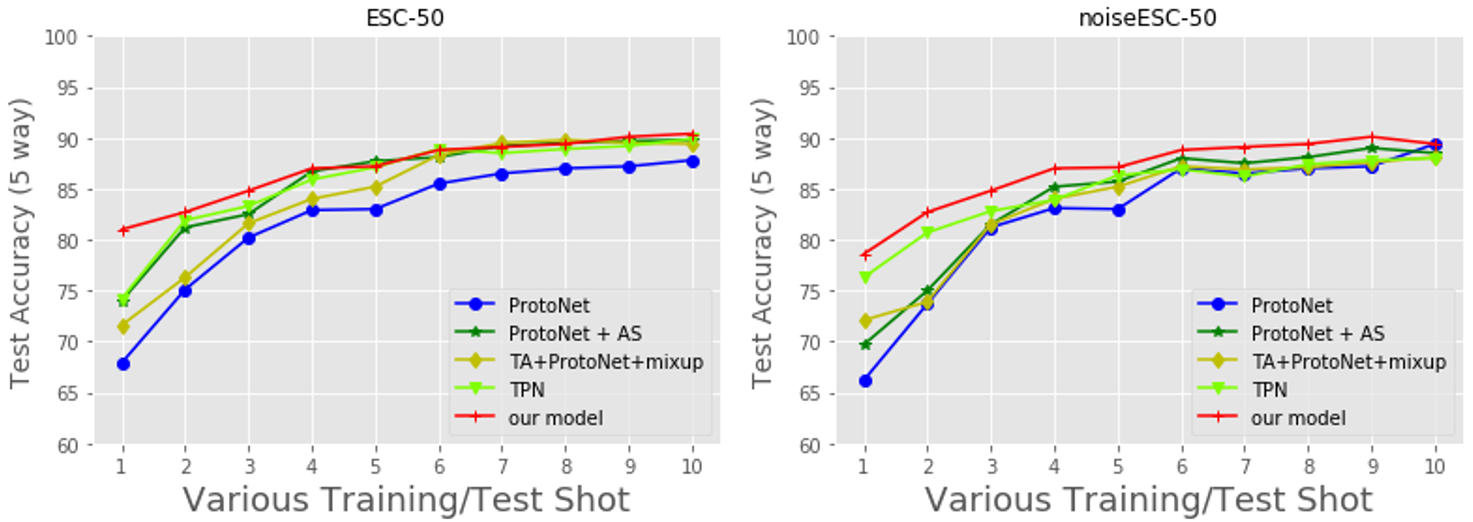
\includegraphics[width=\linewidth]{./pic/exp_8.png}
	\caption{5-way performance with various training/test shots}
	\label{fig:fig_exp_1}
	\vspace{-3mm}
\end{figure}

\subsection{Analysis of domain mismatch}
\vspace{-2mm}
During this subsection, we follow the setting created by~\cite{fewshotdomain}. While the current evaluation focus on recognizing novel class with limited training examples, these novel classes are sampled from the same domain. So, we follow the experiments from~\cite{fewshotdomain}, such a out-of-domain testing could display the ability of few-shot learning methods to generalize~\cite{domainad,domain_ad}. Following the previous setup, the selected AudioSet~\cite{audioSet} with 99 events for meta-train, meta-validation with 21 events and meta-test with 21 events. In addition, the pre-processing are same as the previous description about the setup of~\cite{attentionSimilarity}. The number of ways is set to 5, and we rerun the experiments: ProtoNet, ProtoNet+AS and TPN. For the domain mismatch setting, we experiments "Music" and "Animals" domain as same as~\cite{fewshotdomain}. The events and associated audios from the two domains are removed from train set.

\begin{table}[th]
	\vspace{-3mm}
	\caption{The result of few-shot sound detection in domain mismatch. The AUC(Area Under Curve) is used for evaluation.}
	\label{tab:2}
	\centering
	\scalebox{0.7}{
		\begin{tabular}{l|l|l|l|l|l}
			\toprule
			\multicolumn{2}{l|}{\multirow{2}{*}{Model (AUC)}} & \multicolumn{2}{l|}{1-shot} &  \multicolumn{2}{l}{5-shot} \\ \cline{3-6} 
			\multicolumn{2}{l|}{}  & Music & Animal  & Music & Animal \\ \midrule
			\multicolumn{2}{l|}{ProtoNet\cite{protoNet}}  & 0.712  &  0.644 & 0.824 & 0.729  \\ \midrule
			\multicolumn{2}{l|}{ProtoNet+AS\cite{attentionSimilarity}} & 0.736 & 0.677  & 0.839   & 0.750 \\ \midrule
			\multicolumn{2}{l|}{TPN\cite{TPN}}  & 0.747  & 0.685  & 0.843  & 0.748  \\
			\midrule \midrule
			\multicolumn{2}{l|}{\textbf{\textit{ProtoNet+DA}}}  & 0.752 & 0.680  & 0.836  & 0.739  \\ 
			\midrule
			\multicolumn{2}{l|}{\textbf{\textit{TA+ProtoNet}}}  & 0.759 & 0.691  & 0.851  & 0.763  \\ 
			\midrule
			\multicolumn{2}{l|}{\textbf{\textit{TA+ProtoNet+DA}}}  & 0.762 & 0.694  & 0.854  & 0.761  \\ 
			\midrule
			\multicolumn{2}{l|}{\textbf{\textit{TA+ProtoNet+DA(temporal\&channel)}}}  & \textbf{0.779} & \textbf{0.705}  & \textbf{0.857}  & \textbf{0.768}  \\ 
			\midrule
			\multicolumn{2}{l|}{\textbf{\textit{TPN+DA}}}  & 0.755 & 0.693  & 0.848  & 0.751  \\ 
			\midrule
			\multicolumn{2}{l|}{\textbf{\textit{TA+TPN}}}  & 0.762 & 0.691  & 0.854  & 0.753  \\ 
			\midrule
			\multicolumn{2}{l|}{\textbf{\textit{TA+TPN + DA}}}  & 0.768 & 0.696  & 0.850  & 0.754  \\ 
			\midrule
			\multicolumn{2}{l|}{\textbf{\textit{TA+TPN+DA(temporal\&channel)}}}  & \textbf{0.779} & \textbf{0.705}  & \textbf{0.857}  & \textbf{0.761}  \\ 
			\bottomrule
		\end{tabular}
	\vspace{-3mm}
	}
\end{table}

%\vspace{-4mm}
\section{Conclusion}
%\vspace{-2mm}
In this paper, we proposed a task-adaptive module for few-shot sound event detection. The module contains a task-adaptive extractor (TAE) and a projector. By considering all support examples at same time, TAE could extract the inner-class commonality and the projector could find cross-class characteristic features. Besides, the data augmentation strategy and the novel attention mechanism could further improve model’s performance. We demonstrated that it significantly improved accuracy on two benchmarks (ESC-50 and noiseESC-50), achieving state-of-the-art performance. In addition, we compared with several baselines under the experimental domain mismatch setting, our model could also gain improvement over baselines.

\bibliographystyle{IEEEtran}
\bibliography{mybib}

\end{document}


